\chapter{Background}
\label{chap:Two1}
\section{Data Anonymization}
Training a machine learning classifier requires a huge amount of data however, releasing such amount of person-specific data may pose a huge security risk to indvidual's privacy as it might open them up to Identity fraud,blackmail among other things.
Removing excplicit identifying information such as Names and Email is a solution to prevent information leaking however it must be done in consideration of both the user's privacy and the quality of the data to still be able to use it to in training meaningful prediction models.
\section{Machine Learning} 
Currently one of the trending fields in Artifical Intelligence (AI). Machine learning is generally considered as a subset of AI since it has the ability to learn and act without being
excplicitly programmed. It works by generalizing certian patterns instead of storing the input data and trying to match it exactly\cite{Intro}. For example, building an application to recognize
cats and dogs using Machine Learning can be done by showing the application pictures of different cats and dogs and having the application remember "features" of the cats and dogs to be
able to classify them later on. On the other hand using a traditional approach storing all available pictures of cats and dogs and then later matching pictures exactly with the stored pictures.
\section{Neural Networks}
Neural Networks were introduced in 1943 by Warren McCulloch and Walter Pitts when they presented the first model of the neuron, this discovery ignited the way for research in both biological neural networks and artifical neural networks (ANNs). In the last 10 years however ANNs have been gaining popularity among researchers.\par
ANNs consist of artifical neurons which is modeled after the simplest part of the central nervous system, each neuorn receives input from other neurons which makes them change their state depneding on the input value and finally, produce an output depending on that input and state.\cite{zell1994simulation}
If we look at the network as a whole we will find that it consists of multiple connections, each connection moving the output from neuron $a$ to the next layer in the network to become the input of
neuron $b$ and $b$ is passed onto the next layer as input to $c$ and so on, each of these connections is assigned a weight $w$ that is assigned randomly in the begining then it is iteratively changed, We can also add a bias term if want to influence the outputs to lean onto a certain output that is desirable for us.
\subsection{Fully Connected Neural Networks}
Fully Connected Neural Networks are the most basic neural network, they consist of 3 layers fully interconnected to each other, the three layers are, an inpurt layer, any number of hidden layers and an output layer.
Every neuron starting from the first hidden layers is connected to atleast the following layers and maybe connected to any layer above it. The input is then propagated starting from the input layer until it reaches the output layer, each neuron in every layer has it's own weight,bias values depending on the importance assigned to it by the network.
The activation function of each neuron then decides whether each neuron will be "spiked" or not. The most commonly used activation functions are Sigmoid function, RELU function, Leaky RELU function, Tanh function
\begin{figure}[H]
    \centering
    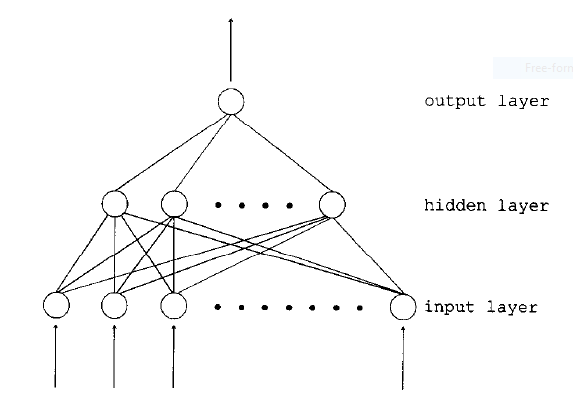
\includegraphics[scale=0.75]{Capture}
    \caption{In the following figure is an example of a fully connected network from \cite{svozil1997introduction}}
    \label{fig:flow}
\end{figure}

\section{Homomorphic Encryption}
After investigating what the latest advances in academic research regarding encryption had reached we came to the conclusion that Homomprhic encryption was the most suitable encryption scheme to use,
To give a brief introduction, Homomorphic encryption is a form of encryption that allows computation on ciphertexts, generating an encrypted result which, when decrypted, matches the result of the operations as if they had been performed on the plaintext.
This makes homomorphic encryption the best candidate in Machine Learning as a service and cloud computing applications.\\
In this study we have compiled the three best implementations of Homomorphic Encryption to the best of our knowledge
\subsection{PALISADE}
Palisade is an open source highly protable cryptography library that supports Homomorphic Encryption. The project was previously funded by the NSA and is developed and maintained by the cryptography
team at New Jersey Institute of Technology. At the time of writing this PALISADE doesn't support floating point operations as it doesn't support CKKS Homomorphic Encryption scheme
\subsection{HELib}
Homomorphic Encryption Library is the second open source library that we looked at, HELib is developed and maintained by Shai Halevi and Victor Shoup.
HELib supports both BGV and CKKS encryption schemes which allows for operations on floating point numbers.
The downside to using HELib is that it less maintained due to the low number of contributors.
\subsection{Microsoft SEAL}
SEAL is a library that is built by Microsoft’s Cryptography team at Microsoft Research\cite{SEAL}. The advantage of SEAL is that it supports both BGV/BFV and CKKS as well being the most documented library of the three.
It also has no dependencies making it modular in addition to having a CMAKE file which is used to build for various environments making it easy to compile and run.\par
It was also demonstrated that SEAL can be used in privacy preserving Machine Learning where the user data was encrypted on-device and the cloud server operated on the encrypted data providing
full user annonymity.
\section{Cross Platform Mobile Development}
The mobile application sector is divided amongst several platforms however the two most dominating platforms are iOS and Android and as a result of this companies need to hire application developers experinced in both platforms or resort to hiring more development teams each assigned to a specific platform which also makes development time longer and causes inconsistency between the different platform applications which might cause user dissatisfaction.
Consequently as a solution, Cross Platform development aims to develop 1 application for multiple platforms having almost the same visual and functional features as native platform applications.\cite{axelsson2016evaluation}
\subsection{React Native}
In 2015 Facebook announced it's new framework React Native which aims to develop native applications for iOS, Android, UWP using the same codebase written in Javascript which reduces the number of developers needed to develop an application and the effort needed for maintainence and code reviews.
React Native also offers the ability to run platform-specific code in Swift, Java, Objective-C.\cite{hansson2016effects} As of 2019, Facebook, Instagram, Uber, Skype and Pintrest are using React Native primarily.